\documentclass[atiam, article]{rapport} % draft, phelma_black, phelma_normal, kit_de, kit_en, phelma_old

\doctitle{TP Cordes}
\title{TP Cordes\\Le ukulélé est-il une petite guitare ?}
\titleheader{TP Cordes}
\titleone{}
\titletwo{Acoustique}
\titlethree{}
\author{Paul Estève, Étienne André, Sébastien Li} % Authors for the header
\autpage{ % Authors for the title page
  \begin{tabular}{l}
    Paul Estève \\
    Étienne André\\
    Sébastien Li
  \end{tabular}
}
\supervisor[Encadrant : ]{Jean-Loïc Le Carrou}
% \supervisorMail{}
\serie{ATIAM 2023/2024}
\date{\today}

\bibliography{biblio}

\begin{document}

\maketitle

\section{Préparation du TP}

On utilise le modèle basse fréquence des instruments de type guitare présenté dans \cite{10.1121/1.384814}.

\begin{figure}
  \begin{center}
    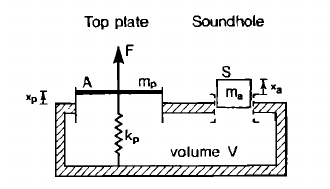
\includegraphics{cordes/schema-modele.png}
  \end{center}
  \caption{Schéma du modèle simplifié en basse fréquence\cite{10.1121/1.384814}}
  \label{fig:schema-bf}
\end{figure}

La table d'harmonie est modélisée par un piston plan de surface équivalente $A$ et de masse $m_p$, lié à une raideur $k_p$. Celui-ci est couplé à l'ensemble {caisse de résonance + évent} modélisé par un résonateur de heimholtz de volume $V$ et de masse acoustique $m_a$ muni d'un trou de surface $S$.

La variation de pression à l'intérieur de la cavité $\Delta p$ est liée à la variation de volume $\Delta V$, dans l'hypothèse de compression adiabatique, par $\Delta p = \frac{-c^2 \rho}{V} \Delta V$ où $c$ est la vitesse du son et $\rho$ la masse volumique de l'air.

On ajoute au modèle les coefficients $R_p$ et $R_a$ représentant les résistances au mouvement du piston et de la masse acoustique.
Le déplacement du piston et de la masse d'air sont notés respectivement $x_p$ et $x_a$, relativement à leur position d'équilibre. Ils sont régis par le système d'équations:

\begin{equation}
  \begin{cases}
    m_p \ddot{x_p} = F - k_p x_p - R_p \dot{x_p} + A \Delta p  \\
    m_a \ddot{x_a} = S \Delta p - R_a \dot{x_a}    
  \end{cases}
\end{equation}

Dans la suite, on cherchera à identifier et comparer les paramètres équivalents de ce modèle sur la guitare et l'ukulélé, en suivant le protocole décrit dans \cite{10.1121/1.384814}.

\section{Protocole de mesure}

\begin{figure}
  \begin{center}
    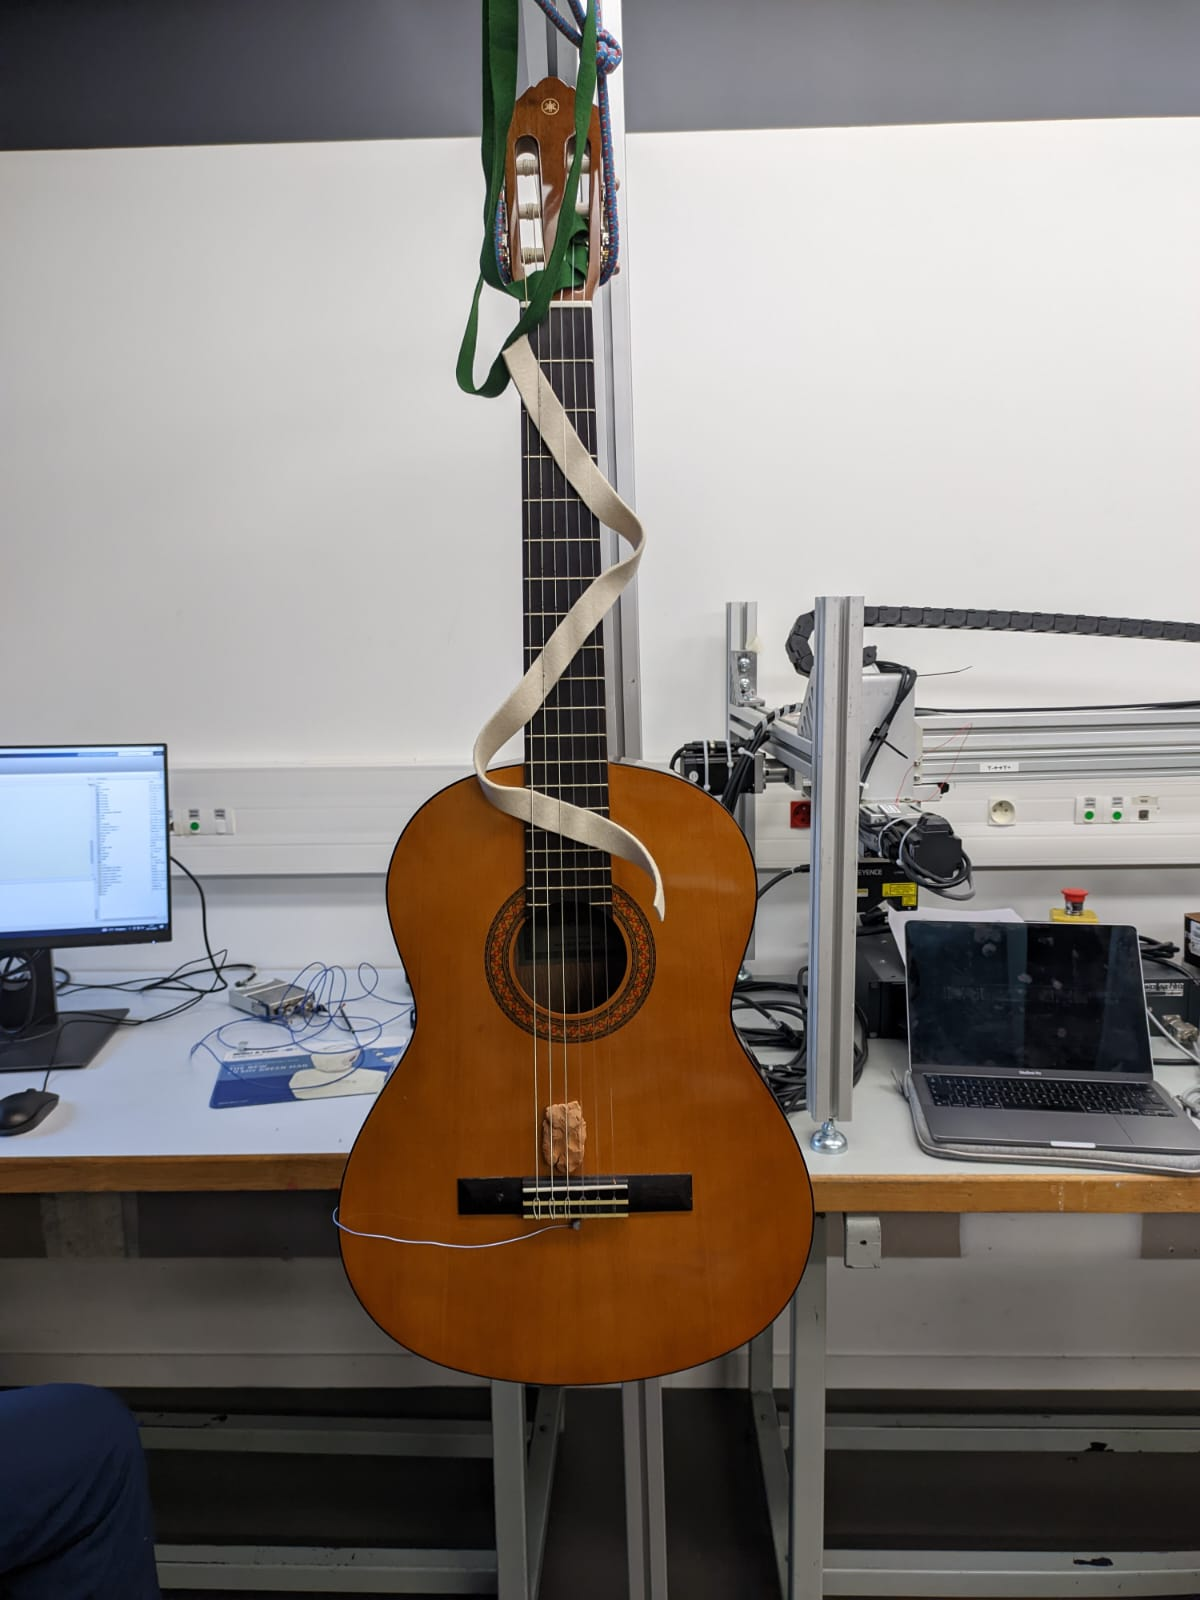
\includegraphics[width=\textwidth/4]{cordes/guitare.jpg}
  \end{center}
  \caption{Guitare en situation de mesure avec masse ajoutée}
  \label{fig:photo-guitare}
\end{figure}
\begin{figure}
  \begin{center}
    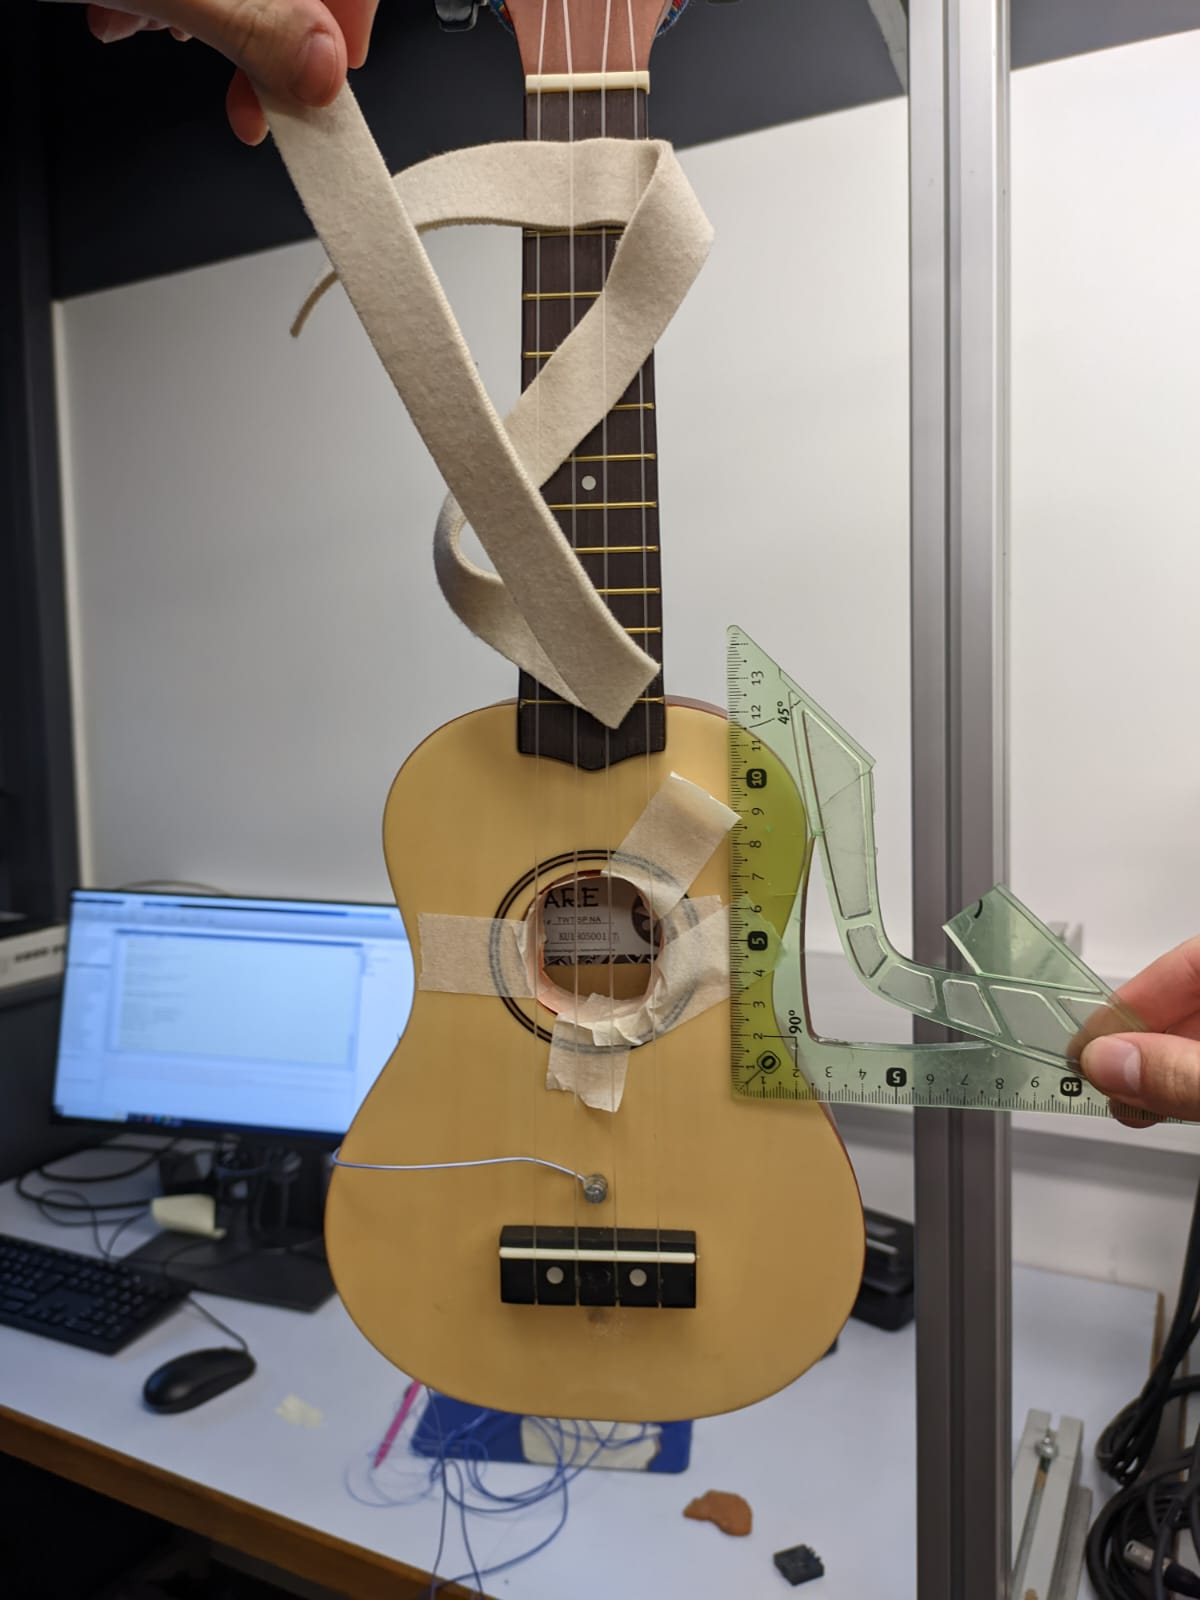
\includegraphics[width=\textwidth/4]{cordes/ukulele.jpg}
  \end{center}
  \caption{Guitare en situation de mesure avec col}
  \label{fig:photo-ukulele}
\end{figure}

On suspend l'instrument à un bras de façon à ce qu'il ne soit pas amorti. On fait également glisser une bande de feutre dans les cordes, afin de les étouffer totalement. On peut voir les deux instruments en situation de mesure aux figures \ref{fig:photo-guitare}.et \ref{fig:photo-ukulele}.

Un accéléromètre est fixé au point de déplacement maximal de la table d'harmonie décrit dans \cite{fletcher2012physics}, juste au-dessous du chevalet pour la guitare et juste au-dessus pour le ukulele, sur l'axe de symétrie de l'instrument. Muni d'un marteau de mesure, on frappe le plus proche possible de ce point, également sur l'axe de symétrie.


Pour chacun des instruments, on effectue 4 mesures :
\begin{enumerate}
    \item Instrument sans modifications
    \item Instrument avec masse ajoutée, sous la forme d'un peu de pâte à modeler fixée sur l'axe de symétrie proche de l'accéléromètre
    \item Instrument avec évent bouché par du papier
    \item Instrument avec col de papier autour de l'évent à l'intérieur de la caisse de résonance.
\end{enumerate}

On veillera à ce que chaque mesure respecte les critères suivants:

\begin{itemize}
    \item La phase de la fonction de transfert doit être comprise entre $0$ et $-\pi$ pour assurer la colocalisation du point de frappe et de mesure de l'accélération.
    \item L'excitation doit être le plus proche possible d'un Dirac afin d'exciter une large gamme de fréquence, et surtout pour éviter les coups doubles.\item L'amplitude de l'excitation doit être suffisament grande pour obtenir des mesures représentatives, mais assez faible pour ne pas endommager le matériel.
\end{itemize}

Un programme MATLAB calcule la fonction de transfert entre le marteau et l'accéléromètre.

Ensuite, un programme python effectue les traitements suivants:
\begin{itemize}
    \item identification des pics et antipics de résonance des fonctions de transfert (via le passage à $-\pi/2$ de la phase)
    \item extraction de leur fréquence, largeur et amplitude
    \item tracé de diverses comparaisons de fonctions de transfert
    \item dérivation des paramètres du modèle en fonction des propriété des pics
    \item simulation du modèle théorique avec les paramètres
    \item comparaison avec la mesure
\end{itemize}

On définit les paramètres expérimentaux suivants, en suivant les notations de \cite{10.1121/1.384814}:
\begin{itemize}
    \item les deux premières fréquences de résonance $f_-$ et $f_+$ de la guitare
    \item la fréquence de résonance du résonateur de helmholtz $f_h$
    \item la masse ajoutée $m_{ajout}$
\end{itemize}

\section{Mesures sur la guitare}
On effectue les 4 premières mesures sur la guitare. Les différentes FRF sont comparées sur les figures \ref{fig:frf-guitare-masse}, \ref{fig:frf-guitare-bouchee} et \ref{fig:frf-guitare-col}. Les pics et antipics sont identifiés à l'aide de croix.

\begin{figure}
    \centering
    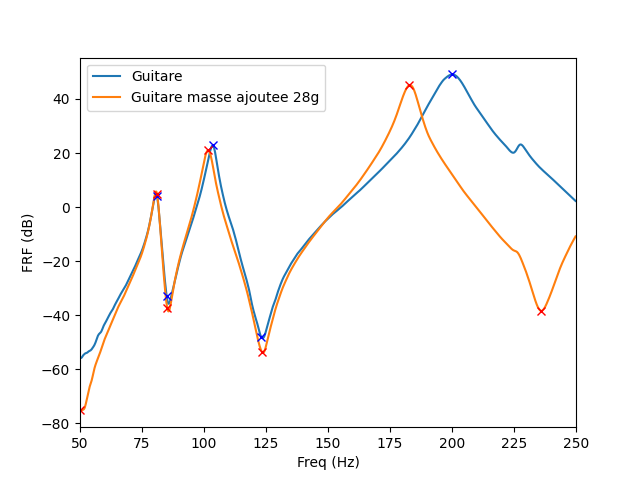
\includegraphics[width=\textwidth]{cordes/images/Guitare masse ajoutee 28g.png}
    \caption{Comparaison des FRF de la guitare nue et avec masse ajoutée}
    \label{fig:frf-guitare-masse}
\end{figure}

\begin{figure}
    \centering
    \includegraphics[width=\textwidth]{cordes/images/Guitare bouchée.png}
    \caption{Comparaison des FRF de la guitare nue et avec évent bouché}
    \label{fig:frf-guitare-bouchee}
\end{figure}

\begin{figure}
    \centering
    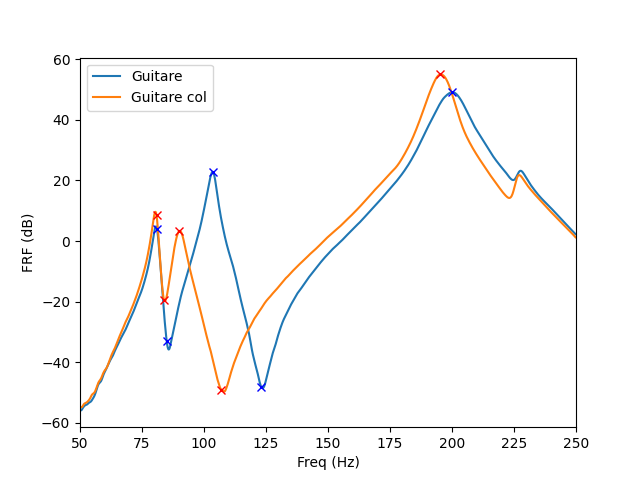
\includegraphics[width=\textwidth]{cordes/images/Guitare col.png}
    \caption{Comparaison des FRF de la guitare nue et avec un col}
    \label{fig:frf-guitare-col}
\end{figure}

On observe plusieurs points:
\begin{itemize}
    \item l'ajout de la masse $m_{ajout} = 28 \si{g}$ (figure \ref{fig:frf-guitare-masse} diminue la fréquence du dernier pic, ce qui permet de l'identifier comme étant la deuxième résonance de la table d'harmonie et d'obtenir $f_+$.
    \item l'obstruction de l'évent (figure \ref{fig:frf-guitare-bouchee}) supprime le deuxième antipic, ce qui permet de l'identifier comme étant la résonance de Helmholtz et d'obtenir $f_h$.
    \item l'ajout d'un col ($4\si{cm}$) abaisse la fréquence de du deuxième pic (car il augmente la masse d'air $m_a$), confirmant le point précédent.
    \item on identifie donc $f_-$ comme étant le premier pic par élimination.
\end{itemize}

\section{Mesures sur le ukulélé}
On procède de même sur le ukulélé.

\begin{figure}
    \centering
    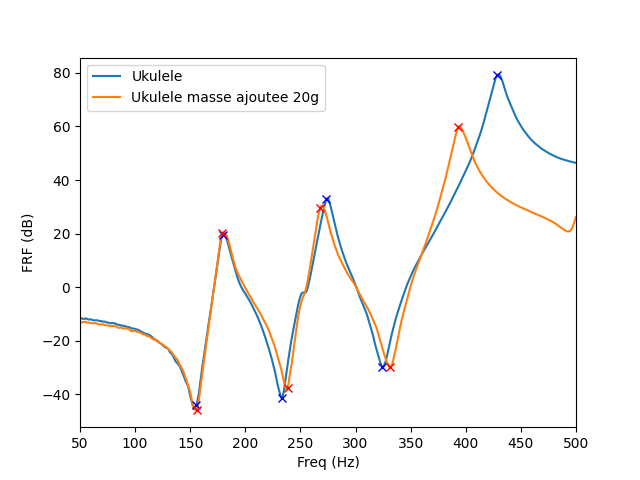
\includegraphics[width=\textwidth]{cordes/images/Ukulele masse ajoutee 20g.png}
    \caption{Comparaison des FRF du ukulélé nu et avec une masse ajoutée}
    \label{fig:enter-label}
\end{figure}

\begin{figure}
    \centering
    \includegraphics[width=\textwidth]{cordes/images/Ukulele bouché.png}
    \caption{Comparaison des FRF du ukulélé nu et avec évent bouché}
    \label{fig:enter-label}
\end{figure}

\begin{figure}
    \centering
    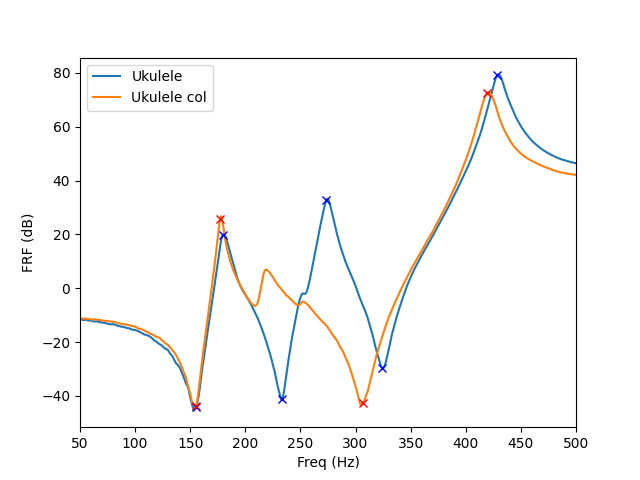
\includegraphics[width=\textwidth]{cordes/images/Ukulele col.png}
    \caption{Comparaison des FRF du ukulélé nu et avec une masse ajoutée}
    \label{fig:enter-label}
\end{figure}

\printbibliography


\end{document}